% Created by tikzDevice version 0.12
% !TEX encoding = UTF-8 Unicode
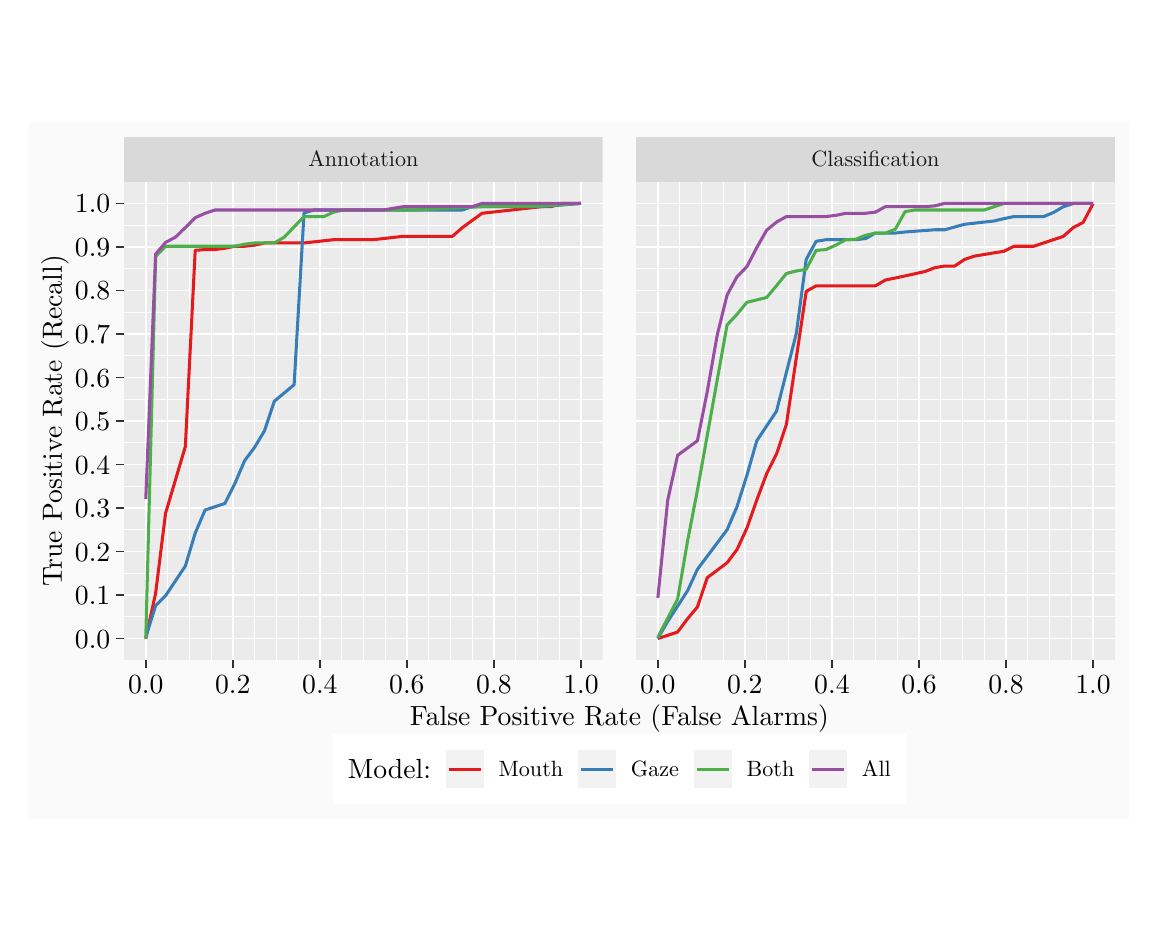
\begin{tikzpicture}[x=1pt,y=1pt]
\definecolor{fillColor}{RGB}{255,255,255}
\path[use as bounding box,fill=fillColor,fill opacity=0.00] (0,0) rectangle (398.34,320.03);
\begin{scope}
\path[clip] (  0.00, 33.88) rectangle (398.34,286.15);
\definecolor{drawColor}{RGB}{255,255,255}
\definecolor{fillColor}{gray}{0.98}

\path[draw=drawColor,line width= 0.6pt,line join=round,line cap=round,fill=fillColor] (  0.00, 33.88) rectangle (398.34,286.15);
\end{scope}
\begin{scope}
\path[clip] ( 34.81, 91.40) rectangle (207.80,264.39);
\definecolor{fillColor}{gray}{0.92}

\path[fill=fillColor] ( 34.81, 91.40) rectangle (207.80,264.39);
\definecolor{drawColor}{RGB}{255,255,255}

\path[draw=drawColor,line width= 0.3pt,line join=round] ( 34.81,107.13) --
	(207.80,107.13);

\path[draw=drawColor,line width= 0.3pt,line join=round] ( 34.81,122.85) --
	(207.80,122.85);

\path[draw=drawColor,line width= 0.3pt,line join=round] ( 34.81,138.58) --
	(207.80,138.58);

\path[draw=drawColor,line width= 0.3pt,line join=round] ( 34.81,154.31) --
	(207.80,154.31);

\path[draw=drawColor,line width= 0.3pt,line join=round] ( 34.81,170.03) --
	(207.80,170.03);

\path[draw=drawColor,line width= 0.3pt,line join=round] ( 34.81,185.76) --
	(207.80,185.76);

\path[draw=drawColor,line width= 0.3pt,line join=round] ( 34.81,201.49) --
	(207.80,201.49);

\path[draw=drawColor,line width= 0.3pt,line join=round] ( 34.81,217.21) --
	(207.80,217.21);

\path[draw=drawColor,line width= 0.3pt,line join=round] ( 34.81,232.94) --
	(207.80,232.94);

\path[draw=drawColor,line width= 0.3pt,line join=round] ( 34.81,248.67) --
	(207.80,248.67);

\path[draw=drawColor,line width= 0.3pt,line join=round] ( 50.53, 91.40) --
	( 50.53,264.39);

\path[draw=drawColor,line width= 0.3pt,line join=round] ( 58.40, 91.40) --
	( 58.40,264.39);

\path[draw=drawColor,line width= 0.3pt,line join=round] ( 66.26, 91.40) --
	( 66.26,264.39);

\path[draw=drawColor,line width= 0.3pt,line join=round] ( 81.99, 91.40) --
	( 81.99,264.39);

\path[draw=drawColor,line width= 0.3pt,line join=round] ( 89.85, 91.40) --
	( 89.85,264.39);

\path[draw=drawColor,line width= 0.3pt,line join=round] ( 97.71, 91.40) --
	( 97.71,264.39);

\path[draw=drawColor,line width= 0.3pt,line join=round] (113.44, 91.40) --
	(113.44,264.39);

\path[draw=drawColor,line width= 0.3pt,line join=round] (121.30, 91.40) --
	(121.30,264.39);

\path[draw=drawColor,line width= 0.3pt,line join=round] (129.17, 91.40) --
	(129.17,264.39);

\path[draw=drawColor,line width= 0.3pt,line join=round] (144.89, 91.40) --
	(144.89,264.39);

\path[draw=drawColor,line width= 0.3pt,line join=round] (152.76, 91.40) --
	(152.76,264.39);

\path[draw=drawColor,line width= 0.3pt,line join=round] (160.62, 91.40) --
	(160.62,264.39);

\path[draw=drawColor,line width= 0.3pt,line join=round] (176.35, 91.40) --
	(176.35,264.39);

\path[draw=drawColor,line width= 0.3pt,line join=round] (184.21, 91.40) --
	(184.21,264.39);

\path[draw=drawColor,line width= 0.3pt,line join=round] (192.07, 91.40) --
	(192.07,264.39);

\path[draw=drawColor,line width= 0.6pt,line join=round] ( 34.81, 99.26) --
	(207.80, 99.26);

\path[draw=drawColor,line width= 0.6pt,line join=round] ( 34.81,114.99) --
	(207.80,114.99);

\path[draw=drawColor,line width= 0.6pt,line join=round] ( 34.81,130.72) --
	(207.80,130.72);

\path[draw=drawColor,line width= 0.6pt,line join=round] ( 34.81,146.44) --
	(207.80,146.44);

\path[draw=drawColor,line width= 0.6pt,line join=round] ( 34.81,162.17) --
	(207.80,162.17);

\path[draw=drawColor,line width= 0.6pt,line join=round] ( 34.81,177.90) --
	(207.80,177.90);

\path[draw=drawColor,line width= 0.6pt,line join=round] ( 34.81,193.62) --
	(207.80,193.62);

\path[draw=drawColor,line width= 0.6pt,line join=round] ( 34.81,209.35) --
	(207.80,209.35);

\path[draw=drawColor,line width= 0.6pt,line join=round] ( 34.81,225.08) --
	(207.80,225.08);

\path[draw=drawColor,line width= 0.6pt,line join=round] ( 34.81,240.80) --
	(207.80,240.80);

\path[draw=drawColor,line width= 0.6pt,line join=round] ( 34.81,256.53) --
	(207.80,256.53);

\path[draw=drawColor,line width= 0.6pt,line join=round] ( 42.67, 91.40) --
	( 42.67,264.39);

\path[draw=drawColor,line width= 0.6pt,line join=round] ( 74.12, 91.40) --
	( 74.12,264.39);

\path[draw=drawColor,line width= 0.6pt,line join=round] (105.58, 91.40) --
	(105.58,264.39);

\path[draw=drawColor,line width= 0.6pt,line join=round] (137.03, 91.40) --
	(137.03,264.39);

\path[draw=drawColor,line width= 0.6pt,line join=round] (168.48, 91.40) --
	(168.48,264.39);

\path[draw=drawColor,line width= 0.6pt,line join=round] (199.94, 91.40) --
	(199.94,264.39);
\definecolor{drawColor}{RGB}{228,26,28}

\path[draw=drawColor,line width= 1.1pt,line join=round] ( 42.67, 99.26) --
	( 46.24,115.70) --
	( 49.82,144.54) --
	( 56.97,168.66) --
	( 60.54,239.57) --
	( 64.11,239.85) --
	( 67.69,239.85) --
	( 71.26,240.33) --
	( 74.84,241.04) --
	( 78.41,241.04) --
	( 81.99,241.44) --
	( 85.56,242.23) --
	( 89.13,242.23) --
	( 92.71,242.23) --
	( 99.86,242.23) --
	(110.58,243.42) --
	(114.15,243.42) --
	(117.73,243.42) --
	(121.30,243.42) --
	(124.88,243.42) --
	(135.60,244.62) --
	(139.17,244.62) --
	(142.75,244.62) --
	(146.32,244.62) --
	(149.90,244.62) --
	(153.47,244.62) --
	(157.05,247.76) --
	(164.19,252.96) --
	(174.92,254.15) --
	(185.64,255.34) --
	(189.21,255.34) --
	(192.79,256.53) --
	(196.36,256.53) --
	(199.94,256.53);
\definecolor{drawColor}{RGB}{55,126,184}

\path[draw=drawColor,line width= 1.1pt,line join=round] ( 42.67, 99.76) --
	( 46.24,111.18) --
	( 49.82,114.75) --
	( 56.97,125.47) --
	( 60.54,137.39) --
	( 64.11,145.73) --
	( 71.26,148.11) --
	( 74.84,155.26) --
	( 78.41,163.60) --
	( 81.99,168.36) --
	( 85.56,174.32) --
	( 89.13,185.04) --
	( 96.28,191.00) --
	( 99.86,253.08) --
	(103.43,254.15) --
	(107.01,254.15) --
	(114.15,254.15) --
	(117.73,254.15) --
	(124.88,254.15) --
	(132.03,254.15) --
	(139.17,254.15) --
	(142.75,254.15) --
	(146.32,254.15) --
	(153.47,254.15) --
	(157.05,254.15) --
	(160.62,255.34) --
	(164.19,255.34) --
	(171.34,255.34) --
	(178.49,255.34) --
	(185.64,255.34) --
	(192.79,255.93) --
	(199.94,256.53);
\definecolor{drawColor}{RGB}{77,175,74}

\path[draw=drawColor,line width= 1.1pt,line join=round] ( 42.67, 99.26) --
	( 46.24,237.36) --
	( 49.82,241.04) --
	( 53.39,241.04) --
	( 56.97,241.04) --
	( 67.69,241.04) --
	( 71.26,241.04) --
	( 74.84,241.04) --
	( 78.41,241.79) --
	( 81.99,242.23) --
	( 85.56,242.23) --
	( 89.13,242.23) --
	( 92.71,244.32) --
	( 96.28,248.07) --
	( 99.86,251.76) --
	(103.43,251.76) --
	(107.01,251.76) --
	(110.58,253.39) --
	(114.15,254.15) --
	(124.88,254.15) --
	(139.17,254.15) --
	(164.19,255.34) --
	(182.07,255.34) --
	(199.94,256.53);
\definecolor{drawColor}{RGB}{152,78,163}

\path[draw=drawColor,line width= 1.1pt,line join=round] ( 42.67,149.70) --
	( 46.24,238.22) --
	( 49.82,242.43) --
	( 53.39,244.32) --
	( 56.97,247.79) --
	( 60.54,251.37) --
	( 64.11,252.96) --
	( 67.69,254.15) --
	( 71.26,254.15) --
	( 74.84,254.15) --
	( 78.41,254.15) --
	( 81.99,254.15) --
	( 92.71,254.15) --
	( 96.28,254.15) --
	( 99.86,254.15) --
	(103.43,254.15) --
	(107.01,254.15) --
	(117.73,254.15) --
	(121.30,254.15) --
	(128.45,254.15) --
	(135.60,255.34) --
	(146.32,255.34) --
	(160.62,255.34) --
	(164.19,256.53) --
	(167.77,256.53) --
	(199.94,256.53);
\end{scope}
\begin{scope}
\path[clip] (219.84, 91.40) rectangle (392.84,264.39);
\definecolor{fillColor}{gray}{0.92}

\path[fill=fillColor] (219.84, 91.40) rectangle (392.84,264.39);
\definecolor{drawColor}{RGB}{255,255,255}

\path[draw=drawColor,line width= 0.3pt,line join=round] (219.84,107.13) --
	(392.84,107.13);

\path[draw=drawColor,line width= 0.3pt,line join=round] (219.84,122.85) --
	(392.84,122.85);

\path[draw=drawColor,line width= 0.3pt,line join=round] (219.84,138.58) --
	(392.84,138.58);

\path[draw=drawColor,line width= 0.3pt,line join=round] (219.84,154.31) --
	(392.84,154.31);

\path[draw=drawColor,line width= 0.3pt,line join=round] (219.84,170.03) --
	(392.84,170.03);

\path[draw=drawColor,line width= 0.3pt,line join=round] (219.84,185.76) --
	(392.84,185.76);

\path[draw=drawColor,line width= 0.3pt,line join=round] (219.84,201.49) --
	(392.84,201.49);

\path[draw=drawColor,line width= 0.3pt,line join=round] (219.84,217.21) --
	(392.84,217.21);

\path[draw=drawColor,line width= 0.3pt,line join=round] (219.84,232.94) --
	(392.84,232.94);

\path[draw=drawColor,line width= 0.3pt,line join=round] (219.84,248.67) --
	(392.84,248.67);

\path[draw=drawColor,line width= 0.3pt,line join=round] (235.57, 91.40) --
	(235.57,264.39);

\path[draw=drawColor,line width= 0.3pt,line join=round] (243.43, 91.40) --
	(243.43,264.39);

\path[draw=drawColor,line width= 0.3pt,line join=round] (251.30, 91.40) --
	(251.30,264.39);

\path[draw=drawColor,line width= 0.3pt,line join=round] (267.02, 91.40) --
	(267.02,264.39);

\path[draw=drawColor,line width= 0.3pt,line join=round] (274.89, 91.40) --
	(274.89,264.39);

\path[draw=drawColor,line width= 0.3pt,line join=round] (282.75, 91.40) --
	(282.75,264.39);

\path[draw=drawColor,line width= 0.3pt,line join=round] (298.48, 91.40) --
	(298.48,264.39);

\path[draw=drawColor,line width= 0.3pt,line join=round] (306.34, 91.40) --
	(306.34,264.39);

\path[draw=drawColor,line width= 0.3pt,line join=round] (314.21, 91.40) --
	(314.21,264.39);

\path[draw=drawColor,line width= 0.3pt,line join=round] (329.93, 91.40) --
	(329.93,264.39);

\path[draw=drawColor,line width= 0.3pt,line join=round] (337.80, 91.40) --
	(337.80,264.39);

\path[draw=drawColor,line width= 0.3pt,line join=round] (345.66, 91.40) --
	(345.66,264.39);

\path[draw=drawColor,line width= 0.3pt,line join=round] (361.39, 91.40) --
	(361.39,264.39);

\path[draw=drawColor,line width= 0.3pt,line join=round] (369.25, 91.40) --
	(369.25,264.39);

\path[draw=drawColor,line width= 0.3pt,line join=round] (377.11, 91.40) --
	(377.11,264.39);

\path[draw=drawColor,line width= 0.6pt,line join=round] (219.84, 99.26) --
	(392.84, 99.26);

\path[draw=drawColor,line width= 0.6pt,line join=round] (219.84,114.99) --
	(392.84,114.99);

\path[draw=drawColor,line width= 0.6pt,line join=round] (219.84,130.72) --
	(392.84,130.72);

\path[draw=drawColor,line width= 0.6pt,line join=round] (219.84,146.44) --
	(392.84,146.44);

\path[draw=drawColor,line width= 0.6pt,line join=round] (219.84,162.17) --
	(392.84,162.17);

\path[draw=drawColor,line width= 0.6pt,line join=round] (219.84,177.90) --
	(392.84,177.90);

\path[draw=drawColor,line width= 0.6pt,line join=round] (219.84,193.62) --
	(392.84,193.62);

\path[draw=drawColor,line width= 0.6pt,line join=round] (219.84,209.35) --
	(392.84,209.35);

\path[draw=drawColor,line width= 0.6pt,line join=round] (219.84,225.08) --
	(392.84,225.08);

\path[draw=drawColor,line width= 0.6pt,line join=round] (219.84,240.80) --
	(392.84,240.80);

\path[draw=drawColor,line width= 0.6pt,line join=round] (219.84,256.53) --
	(392.84,256.53);

\path[draw=drawColor,line width= 0.6pt,line join=round] (227.71, 91.40) --
	(227.71,264.39);

\path[draw=drawColor,line width= 0.6pt,line join=round] (259.16, 91.40) --
	(259.16,264.39);

\path[draw=drawColor,line width= 0.6pt,line join=round] (290.61, 91.40) --
	(290.61,264.39);

\path[draw=drawColor,line width= 0.6pt,line join=round] (322.07, 91.40) --
	(322.07,264.39);

\path[draw=drawColor,line width= 0.6pt,line join=round] (353.52, 91.40) --
	(353.52,264.39);

\path[draw=drawColor,line width= 0.6pt,line join=round] (384.98, 91.40) --
	(384.98,264.39);
\definecolor{drawColor}{RGB}{228,26,28}

\path[draw=drawColor,line width= 1.1pt,line join=round] (227.71, 99.29) --
	(231.28,100.45) --
	(234.86,101.65) --
	(238.43,106.41) --
	(242.01,110.70) --
	(245.58,121.30) --
	(252.73,126.67) --
	(256.30,131.43) --
	(259.88,139.18) --
	(263.45,149.30) --
	(267.02,158.83) --
	(270.60,165.98) --
	(274.17,176.70) --
	(281.32,224.73) --
	(284.90,226.74) --
	(288.47,226.74) --
	(292.04,226.74) --
	(295.62,226.74) --
	(302.77,226.74) --
	(306.34,226.74) --
	(309.92,228.83) --
	(317.06,230.32) --
	(324.21,231.91) --
	(327.79,233.30) --
	(331.36,233.89) --
	(334.94,233.89) --
	(338.51,236.28) --
	(342.08,237.47) --
	(349.23,238.66) --
	(352.81,239.25) --
	(356.38,241.04) --
	(359.96,241.04) --
	(363.53,241.04) --
	(367.10,242.23) --
	(370.68,243.42) --
	(374.25,244.62) --
	(377.83,247.79) --
	(381.40,249.68) --
	(384.98,256.41);
\definecolor{drawColor}{RGB}{55,126,184}

\path[draw=drawColor,line width= 1.1pt,line join=round] (227.71, 99.36) --
	(231.28,105.46) --
	(238.43,116.54) --
	(242.01,124.28) --
	(245.58,129.05) --
	(252.73,138.58) --
	(256.30,146.92) --
	(259.88,158.24) --
	(263.45,170.75) --
	(270.60,181.47) --
	(277.75,209.55) --
	(281.32,236.28) --
	(284.90,242.83) --
	(288.47,243.42) --
	(292.04,243.42) --
	(299.19,243.42) --
	(302.77,243.82) --
	(306.34,245.81) --
	(313.49,245.81) --
	(317.06,246.20) --
	(327.79,247.00) --
	(331.36,247.00) --
	(338.51,248.98) --
	(349.23,250.18) --
	(352.81,251.05) --
	(356.38,251.76) --
	(359.96,251.76) --
	(367.10,251.76) --
	(370.68,253.25) --
	(374.25,255.34) --
	(377.83,256.53) --
	(381.40,256.53) --
	(384.98,256.53);
\definecolor{drawColor}{RGB}{77,175,74}

\path[draw=drawColor,line width= 1.1pt,line join=round] (227.71, 99.80) --
	(234.86,113.56) --
	(238.43,134.41) --
	(242.01,152.88) --
	(252.73,212.62) --
	(256.30,216.42) --
	(259.88,220.79) --
	(267.02,222.52) --
	(270.60,226.83) --
	(274.17,231.21) --
	(277.75,232.11) --
	(281.32,232.70) --
	(284.90,239.55) --
	(288.47,239.85) --
	(292.04,241.47) --
	(295.62,243.42) --
	(299.19,243.57) --
	(302.77,245.01) --
	(306.34,245.81) --
	(309.92,245.81) --
	(313.49,247.17) --
	(317.06,253.57) --
	(320.64,254.15) --
	(324.21,254.15) --
	(327.79,254.15) --
	(331.36,254.15) --
	(338.51,254.15) --
	(342.08,254.15) --
	(345.66,254.15) --
	(349.23,255.34) --
	(352.81,256.53) --
	(356.38,256.53) --
	(359.96,256.53) --
	(363.53,256.53) --
	(370.68,256.53) --
	(374.25,256.53) --
	(377.83,256.53) --
	(381.40,256.53) --
	(384.98,256.53);
\definecolor{drawColor}{RGB}{152,78,163}

\path[draw=drawColor,line width= 1.1pt,line join=round] (227.71,113.96) --
	(231.28,149.30) --
	(234.86,165.51) --
	(242.01,170.75) --
	(245.58,188.62) --
	(249.15,208.87) --
	(252.73,223.42) --
	(256.30,230.02) --
	(259.88,233.66) --
	(263.45,240.54) --
	(267.02,246.83) --
	(270.60,249.79) --
	(274.17,251.76) --
	(277.75,251.76) --
	(281.32,251.76) --
	(284.90,251.76) --
	(288.47,251.76) --
	(292.04,252.21) --
	(295.62,252.96) --
	(302.77,252.96) --
	(306.34,253.38) --
	(309.92,255.34) --
	(313.49,255.34) --
	(317.06,255.34) --
	(320.64,255.34) --
	(324.21,255.34) --
	(327.79,255.64) --
	(331.36,256.53) --
	(334.94,256.53) --
	(338.51,256.53) --
	(345.66,256.53) --
	(352.81,256.53) --
	(356.38,256.53) --
	(359.96,256.53) --
	(367.10,256.53) --
	(377.83,256.53) --
	(384.98,256.53);
\end{scope}
\begin{scope}
\path[clip] ( 34.81,264.39) rectangle (207.80,280.65);
\definecolor{fillColor}{gray}{0.85}

\path[fill=fillColor] ( 34.81,264.39) rectangle (207.80,280.65);
\definecolor{drawColor}{gray}{0.10}

\node[text=drawColor,anchor=base,inner sep=0pt, outer sep=0pt, scale=  0.80] at (121.30,269.77) {Annotation};
\end{scope}
\begin{scope}
\path[clip] (219.84,264.39) rectangle (392.84,280.65);
\definecolor{fillColor}{gray}{0.85}

\path[fill=fillColor] (219.84,264.39) rectangle (392.84,280.65);
\definecolor{drawColor}{gray}{0.10}

\node[text=drawColor,anchor=base,inner sep=0pt, outer sep=0pt, scale=  0.80] at (306.34,269.77) {Classification};
\end{scope}
\begin{scope}
\path[clip] (  0.00,  0.00) rectangle (398.34,320.03);
\definecolor{drawColor}{gray}{0.20}

\path[draw=drawColor,line width= 0.6pt,line join=round] ( 42.67, 88.65) --
	( 42.67, 91.40);

\path[draw=drawColor,line width= 0.6pt,line join=round] ( 74.12, 88.65) --
	( 74.12, 91.40);

\path[draw=drawColor,line width= 0.6pt,line join=round] (105.58, 88.65) --
	(105.58, 91.40);

\path[draw=drawColor,line width= 0.6pt,line join=round] (137.03, 88.65) --
	(137.03, 91.40);

\path[draw=drawColor,line width= 0.6pt,line join=round] (168.48, 88.65) --
	(168.48, 91.40);

\path[draw=drawColor,line width= 0.6pt,line join=round] (199.94, 88.65) --
	(199.94, 91.40);
\end{scope}
\begin{scope}
\path[clip] (  0.00,  0.00) rectangle (398.34,320.03);
\definecolor{drawColor}{RGB}{0,0,0}

\node[text=drawColor,anchor=base,inner sep=0pt, outer sep=0pt, scale=  1.00] at ( 42.67, 79.56) {0.0};

\node[text=drawColor,anchor=base,inner sep=0pt, outer sep=0pt, scale=  1.00] at ( 74.12, 79.56) {0.2};

\node[text=drawColor,anchor=base,inner sep=0pt, outer sep=0pt, scale=  1.00] at (105.58, 79.56) {0.4};

\node[text=drawColor,anchor=base,inner sep=0pt, outer sep=0pt, scale=  1.00] at (137.03, 79.56) {0.6};

\node[text=drawColor,anchor=base,inner sep=0pt, outer sep=0pt, scale=  1.00] at (168.48, 79.56) {0.8};

\node[text=drawColor,anchor=base,inner sep=0pt, outer sep=0pt, scale=  1.00] at (199.94, 79.56) {1.0};
\end{scope}
\begin{scope}
\path[clip] (  0.00,  0.00) rectangle (398.34,320.03);
\definecolor{drawColor}{gray}{0.20}

\path[draw=drawColor,line width= 0.6pt,line join=round] (227.71, 88.65) --
	(227.71, 91.40);

\path[draw=drawColor,line width= 0.6pt,line join=round] (259.16, 88.65) --
	(259.16, 91.40);

\path[draw=drawColor,line width= 0.6pt,line join=round] (290.61, 88.65) --
	(290.61, 91.40);

\path[draw=drawColor,line width= 0.6pt,line join=round] (322.07, 88.65) --
	(322.07, 91.40);

\path[draw=drawColor,line width= 0.6pt,line join=round] (353.52, 88.65) --
	(353.52, 91.40);

\path[draw=drawColor,line width= 0.6pt,line join=round] (384.98, 88.65) --
	(384.98, 91.40);
\end{scope}
\begin{scope}
\path[clip] (  0.00,  0.00) rectangle (398.34,320.03);
\definecolor{drawColor}{RGB}{0,0,0}

\node[text=drawColor,anchor=base,inner sep=0pt, outer sep=0pt, scale=  1.00] at (227.71, 79.56) {0.0};

\node[text=drawColor,anchor=base,inner sep=0pt, outer sep=0pt, scale=  1.00] at (259.16, 79.56) {0.2};

\node[text=drawColor,anchor=base,inner sep=0pt, outer sep=0pt, scale=  1.00] at (290.61, 79.56) {0.4};

\node[text=drawColor,anchor=base,inner sep=0pt, outer sep=0pt, scale=  1.00] at (322.07, 79.56) {0.6};

\node[text=drawColor,anchor=base,inner sep=0pt, outer sep=0pt, scale=  1.00] at (353.52, 79.56) {0.8};

\node[text=drawColor,anchor=base,inner sep=0pt, outer sep=0pt, scale=  1.00] at (384.98, 79.56) {1.0};
\end{scope}
\begin{scope}
\path[clip] (  0.00,  0.00) rectangle (398.34,320.03);
\definecolor{drawColor}{RGB}{0,0,0}

\node[text=drawColor,anchor=base east,inner sep=0pt, outer sep=0pt, scale=  1.00] at ( 29.86, 95.82) {0.0};

\node[text=drawColor,anchor=base east,inner sep=0pt, outer sep=0pt, scale=  1.00] at ( 29.86,111.55) {0.1};

\node[text=drawColor,anchor=base east,inner sep=0pt, outer sep=0pt, scale=  1.00] at ( 29.86,127.27) {0.2};

\node[text=drawColor,anchor=base east,inner sep=0pt, outer sep=0pt, scale=  1.00] at ( 29.86,143.00) {0.3};

\node[text=drawColor,anchor=base east,inner sep=0pt, outer sep=0pt, scale=  1.00] at ( 29.86,158.73) {0.4};

\node[text=drawColor,anchor=base east,inner sep=0pt, outer sep=0pt, scale=  1.00] at ( 29.86,174.45) {0.5};

\node[text=drawColor,anchor=base east,inner sep=0pt, outer sep=0pt, scale=  1.00] at ( 29.86,190.18) {0.6};

\node[text=drawColor,anchor=base east,inner sep=0pt, outer sep=0pt, scale=  1.00] at ( 29.86,205.91) {0.7};

\node[text=drawColor,anchor=base east,inner sep=0pt, outer sep=0pt, scale=  1.00] at ( 29.86,221.63) {0.8};

\node[text=drawColor,anchor=base east,inner sep=0pt, outer sep=0pt, scale=  1.00] at ( 29.86,237.36) {0.9};

\node[text=drawColor,anchor=base east,inner sep=0pt, outer sep=0pt, scale=  1.00] at ( 29.86,253.09) {1.0};
\end{scope}
\begin{scope}
\path[clip] (  0.00,  0.00) rectangle (398.34,320.03);
\definecolor{drawColor}{gray}{0.20}

\path[draw=drawColor,line width= 0.6pt,line join=round] ( 32.06, 99.26) --
	( 34.81, 99.26);

\path[draw=drawColor,line width= 0.6pt,line join=round] ( 32.06,114.99) --
	( 34.81,114.99);

\path[draw=drawColor,line width= 0.6pt,line join=round] ( 32.06,130.72) --
	( 34.81,130.72);

\path[draw=drawColor,line width= 0.6pt,line join=round] ( 32.06,146.44) --
	( 34.81,146.44);

\path[draw=drawColor,line width= 0.6pt,line join=round] ( 32.06,162.17) --
	( 34.81,162.17);

\path[draw=drawColor,line width= 0.6pt,line join=round] ( 32.06,177.90) --
	( 34.81,177.90);

\path[draw=drawColor,line width= 0.6pt,line join=round] ( 32.06,193.62) --
	( 34.81,193.62);

\path[draw=drawColor,line width= 0.6pt,line join=round] ( 32.06,209.35) --
	( 34.81,209.35);

\path[draw=drawColor,line width= 0.6pt,line join=round] ( 32.06,225.08) --
	( 34.81,225.08);

\path[draw=drawColor,line width= 0.6pt,line join=round] ( 32.06,240.80) --
	( 34.81,240.80);

\path[draw=drawColor,line width= 0.6pt,line join=round] ( 32.06,256.53) --
	( 34.81,256.53);
\end{scope}
\begin{scope}
\path[clip] (  0.00,  0.00) rectangle (398.34,320.03);
\definecolor{drawColor}{RGB}{0,0,0}

\node[text=drawColor,anchor=base,inner sep=0pt, outer sep=0pt, scale=  1.00] at (213.82, 67.98) {False Positive Rate (False Alarms)};
\end{scope}
\begin{scope}
\path[clip] (  0.00,  0.00) rectangle (398.34,320.03);
\definecolor{drawColor}{RGB}{0,0,0}

\node[text=drawColor,rotate= 90.00,anchor=base,inner sep=0pt, outer sep=0pt, scale=  1.00] at ( 12.39,177.90) {True Positive Rate (Recall)};
\end{scope}
\begin{scope}
\path[clip] (  0.00,  0.00) rectangle (398.34,320.03);
\definecolor{fillColor}{RGB}{255,255,255}

\path[fill=fillColor] (110.23, 39.38) rectangle (317.41, 64.83);
\end{scope}
\begin{scope}
\path[clip] (  0.00,  0.00) rectangle (398.34,320.03);
\definecolor{drawColor}{RGB}{0,0,0}

\node[text=drawColor,anchor=base west,inner sep=0pt, outer sep=0pt, scale=  1.00] at (115.73, 48.66) {Model:};
\end{scope}
\begin{scope}
\path[clip] (  0.00,  0.00) rectangle (398.34,320.03);
\definecolor{drawColor}{RGB}{255,255,255}
\definecolor{fillColor}{gray}{0.95}

\path[draw=drawColor,line width= 0.6pt,line join=round,line cap=round,fill=fillColor] (150.72, 44.88) rectangle (165.18, 59.33);
\end{scope}
\begin{scope}
\path[clip] (  0.00,  0.00) rectangle (398.34,320.03);
\definecolor{drawColor}{RGB}{228,26,28}

\path[draw=drawColor,line width= 1.1pt,line join=round] (152.17, 52.11) -- (163.73, 52.11);
\end{scope}
\begin{scope}
\path[clip] (  0.00,  0.00) rectangle (398.34,320.03);
\definecolor{drawColor}{RGB}{255,255,255}
\definecolor{fillColor}{gray}{0.95}

\path[draw=drawColor,line width= 0.6pt,line join=round,line cap=round,fill=fillColor] (198.51, 44.88) rectangle (212.96, 59.33);
\end{scope}
\begin{scope}
\path[clip] (  0.00,  0.00) rectangle (398.34,320.03);
\definecolor{drawColor}{RGB}{55,126,184}

\path[draw=drawColor,line width= 1.1pt,line join=round] (199.95, 52.11) -- (211.51, 52.11);
\end{scope}
\begin{scope}
\path[clip] (  0.00,  0.00) rectangle (398.34,320.03);
\definecolor{drawColor}{RGB}{255,255,255}
\definecolor{fillColor}{gray}{0.95}

\path[draw=drawColor,line width= 0.6pt,line join=round,line cap=round,fill=fillColor] (240.34, 44.88) rectangle (254.80, 59.33);
\end{scope}
\begin{scope}
\path[clip] (  0.00,  0.00) rectangle (398.34,320.03);
\definecolor{drawColor}{RGB}{77,175,74}

\path[draw=drawColor,line width= 1.1pt,line join=round] (241.79, 52.11) -- (253.35, 52.11);
\end{scope}
\begin{scope}
\path[clip] (  0.00,  0.00) rectangle (398.34,320.03);
\definecolor{drawColor}{RGB}{255,255,255}
\definecolor{fillColor}{gray}{0.95}

\path[draw=drawColor,line width= 0.6pt,line join=round,line cap=round,fill=fillColor] (282.02, 44.88) rectangle (296.47, 59.33);
\end{scope}
\begin{scope}
\path[clip] (  0.00,  0.00) rectangle (398.34,320.03);
\definecolor{drawColor}{RGB}{152,78,163}

\path[draw=drawColor,line width= 1.1pt,line join=round] (283.46, 52.11) -- (295.03, 52.11);
\end{scope}
\begin{scope}
\path[clip] (  0.00,  0.00) rectangle (398.34,320.03);
\definecolor{drawColor}{RGB}{0,0,0}

\node[text=drawColor,anchor=base west,inner sep=0pt, outer sep=0pt, scale=  0.80] at (170.18, 49.35) {Mouth};
\end{scope}
\begin{scope}
\path[clip] (  0.00,  0.00) rectangle (398.34,320.03);
\definecolor{drawColor}{RGB}{0,0,0}

\node[text=drawColor,anchor=base west,inner sep=0pt, outer sep=0pt, scale=  0.80] at (217.96, 49.35) {Gaze};
\end{scope}
\begin{scope}
\path[clip] (  0.00,  0.00) rectangle (398.34,320.03);
\definecolor{drawColor}{RGB}{0,0,0}

\node[text=drawColor,anchor=base west,inner sep=0pt, outer sep=0pt, scale=  0.80] at (259.80, 49.35) {Both};
\end{scope}
\begin{scope}
\path[clip] (  0.00,  0.00) rectangle (398.34,320.03);
\definecolor{drawColor}{RGB}{0,0,0}

\node[text=drawColor,anchor=base west,inner sep=0pt, outer sep=0pt, scale=  0.80] at (301.47, 49.35) {All};
\end{scope}
\end{tikzpicture}
